% http://www.ctan.org/tex-archive/macros/latex/contrib/beamer/examples
% http://latex.artikel-namsu.de/english/beamer-examples.html

%\documentclass{beamer}
\documentclass[usenames,dvipsnames]{beamer}
\usepackage{amsmath}
\usepackage{amssymb}
\usepackage{bm}
\usepackage{fancybox, graphicx}
\usepackage{listings}
\usepackage{tikz} % Diagrams
\usetikzlibrary {arrows.meta}
\usepackage{color}
\usepackage{textcomp} % See https://tex.stackexchange.com/questions/145416/how-to-have-straight-single-quotes-in-lstlistings

\newcommand{\mathd}{\ensuremath{\mathrm{d}}}

\lstset{language=bash,upquote=true} % Format listings as appropriate for bash. Inexplicably we get problems if the language is set as part of the \begin{lstlisting} command.

% https://tex.stackexchange.com/questions/36030/how-to-make-a-single-word-look-as-some-code
\definecolor{light-gray}{gray}{0.95}
\newcommand{\code}[1]{\colorbox{light-gray}{\texttt{#1}}}
\DeclareMathOperator{\erf}{erf}

\usetheme{boxes}
\usecolortheme{beaver}

\title{What Can a Bayesian Say About $y/x$?}
\author{Lorne Whiteway \\ lorne.whiteway.13@ucl.ac.uk}
\institute{Astrophysics Group \\ Department of Physics and Astronomy \\ University College London}
\date{FLATs \\ 21 November 2025}

\begin{document}

\frame{\titlepage}

\begin{frame}{Purpose of presentation}
  \begin{block}{}
    \begin{itemize}
      \item{I'll show how to do Bayesian inference in a context that is straightforward but non-trivial.}
      \item{Talk will be pedagogical and mostly mathematical.}
      \item{Prior knowledge of Bayesian ideas is useful but not necessary.}
      \item{Thanks to Niall Jeffrey for help.}
    \end{itemize}
  \end{block}
\end{frame}

\begin{frame}{The Original Cosmological Motivation (1)}
  \begin{block}{}
    \begin{itemize}
      \item{The \textit{overdensity} of dark matter (DM), denoted $\delta_{\textrm{DM}}$,  is the percentage difference between the local density (in some volume) and the universal average density. }
      \item{Overdensities have existed since early times. Gravity draws DM into overdense regions, so the overdensities get bigger with time.}
      \item{There is a similar definition for galaxies. Galaxies form in DM overdensities, so we get galaxy overdensities in the same place.}
    \end{itemize}
  \end{block}
\end{frame}

\begin{frame}{The Original Cosmological Motivation (2)}
  \begin{block}{}
    \begin{itemize}
      \item{Physical effects mean that the galaxy overdensity need not equal the DM overdensity; a simple model assumes a linear relationship:
      \begin{equation*}
      b = \frac{\delta_{\textrm{galaxy}}}{\delta_{\textrm{DM}}}
      \end{equation*}
      }
      \medskip
      \item{In a recent paper (\url{https://arxiv.org/abs/2509.18967}), we (Ellen, Niall, LW, Ofer, Josh, et al.) measured the galaxy overdensity (from galaxy counts) and the DM overdensity (from weak-lensing mass maps). But how then to infer something about $b$?}
    \end{itemize}
  \end{block}
\end{frame}

\begin{frame}{Setting up a toy problem}
  \begin{block}{}
    \begin{itemize}
      \item{We make noisy measurements of $x$ and $y$ and we want to infer $b = y/x$.}
      \item{The answer will ideally be a probability distribution for $b$ (and not for example just a single `best' estimate).}
    \end{itemize}
  \end{block}
\end{frame}

\begin{frame}{Noise within the toy problem}
  \begin{block}{}
  \begin{itemize}
    \item{
    Our toy problem has simple measurement noise: \\
    \bigskip
    The measurement noise in $x$ and the measurement noise in $y$ have uncorrelated Gaussian distributions with zero means and unit standard deviations.
    }
    \end{itemize}
  \end{block}
\end{frame}

\begin{frame}{Data within the toy problem}
  \begin{block}{}
  \begin{itemize}
    \item{We make one observation of $x$ (call the measured value $\tilde{x}$) and one of $y$ (call the measured value $\tilde{y}$). \\ \bigskip}
    \item{We measure $\tilde{x} = 3$ and $\tilde{y} = 4$. Signal-to-noise is low!}
    \end{itemize}
  \end{block}
\end{frame}

\begin{frame}{Graph of the observed data}
	\begin{figure}
	\centering
		\includegraphics[scale=0.75]{figure_1.png}
	\end{figure}
\end{frame}

\begin{frame}{Naive calculation}
  \begin{block}{}
    \begin{itemize}
    \item{So here's a naive calculation that appears reasonable to do:}
    \item{By subtracting the (unknown) noise from $(\tilde{x},\tilde{y})$ we get a Gaussian distribution of the true values $(x,y)$ that is centred on $(\tilde{x},\tilde{y})$. For each possible true $(x,y)$ there is a true $b=y/x$, hence we have a distribution $p$ of the true $b$.}
   \end{itemize}
  \end{block}
\end{frame}

\begin{frame}{Naive: scatter of true $x$, $y$ contingent on observed data}
	\begin{figure}
	\centering
		\includegraphics[scale=0.75]{figure_2.png}
	\end{figure}
\end{frame}

\begin{frame}{Naive calculation}
    \begin{itemize}
    \item{In this naive calculation the probability of $b$ is given by the probability mass on a thin pie region (on which $b=y/x$ is constant).}
    \end{itemize}
\end{frame}


\begin{frame}{Naive: count green dots in pie region to get prob of $b$}
	\begin{figure}
	\centering
		\includegraphics[scale=0.75]{figure_3.png}
	\end{figure}
\end{frame}



\begin{frame}{What is the statistical theory behind this calculation?}
    Two main statistical paradigms, with different notions of what `probability' means:
    \begin{itemize}
    \item{Frequentist. Probability is \textit{limiting ratio as the  number of trials goes to infinity} e.g. probability of rolling 8 with two dice is $5/36$. The true value are fixed, and cannot be modelled probabilistically; randomness enters via measurement noise.}
    \item{Bayesian. Probability is \textit{subjective degree of belief} (subjective as it depends on how much information we have). We don't know the true value, hence we can speak probabilistically about it.}
    \end{itemize}
\end{frame}

\begin{frame}{Naive calculation}
        \begin{itemize}
    \item{So the naive calculation can't be frequentist (as it uses the notion of a probability distribution of the true $x$ and $y$). \\ \bigskip}
    \item{So it's Bayesian - but half-baked! Let's do it properly.}
    \end{itemize}
\end{frame}

\begin{frame}{Bayesian theory requires a \textit{model}}
        \begin{itemize}
    \item{This includes a \textit{data model}. The data model will generally go all the way from (at the start) some model parameters, via various calculations (some mathematical, some physical, and certainly some modelling the effect of measurement noise) through to (at the end) observables i.e. measured data.}
    \item{This also includes \textit{prior} results (e.g. from previous experiments) on the probability distributions of the data model parameters.}
    \item{Technically, the model is a specification of the joint distribution of parameters and data $p(\textrm{data}, \textrm{params})$.}
    \item{Can use the model to (e.g.) create new `synthetic' data.}
    \end{itemize}
\end{frame}

\begin{frame}{Bayesian inference}
        \begin{itemize}
    \item{Once we have new data, we use the rules of conditional probability to refine the probability distribution of the data model parameters, moving from the \textit{prior} probability that we had before our experiment to the new \textit{posterior} probability after our experiment.}
    \item{The result from conditional probability is Bayes's Theorem: \\
    \begin{equation*}
    p(\textrm{params}|\textrm{data}) \propto p(\textrm{data} | \textrm{params}) \ p(\textrm{params})
    \end{equation*}
    }
    \item{This gives us the shape of the posterior distribution of the parameters, but not the overall normalisation; in many applications the normalisation doesn't matter.}
    \end{itemize}
\end{frame}

\begin{frame}{Likelihood}
        \begin{itemize}
    \item{The first term on the right hand side, $p(\textrm{data} | \textrm{params})$, is the \textit{likelihood}. It's a probability distribution for the data (e.g. if we integrate over all possible data, with the params held fixed, we will get unity).}
    \item{But we use it \textit{the other way around}: we hold the data fixed, and see how the likelihood varies as the model parameters vary.}
    \end{itemize}
\end{frame}

\begin{frame}{Model for our ratio problem}
        \begin{itemize}
    \item{We are interested in the ratio $b$, so let's make that a model parameter.}
    \item{We need to specify a prior probability distribution for $b$. Here we are departing from the naive calculation; it requires that we \textbf{be physicists} i.e. think about the actual meaning of the ratio. To keep the calculations easy, I make the following prior assumption: $b$ must be positive, and cannot exceed $10$, and the probability is flat between these values (so is a \textit{top hat}).}
    \end{itemize}
\end{frame}

\begin{frame}{A nuisance parameter}
        \begin{itemize}
    \item{Is that enough? Well, can we generate new simulated data observations? No! All we can do is choose a plausable value of $b$ from our prior distribution; that's not enough to generate new simulated data, as we have no idea what $x$ and $y$ need to be.}
    \item{So we need at least one new parameter. It will suffice e.g. to take $x$ as a parameter. This is a \textit{nuisance} parameter; it's needed but we don't actually care about its value. We also need a prior distribution on $x$; again here we need to know that actual physical meaning of $x$. For simplicity I will take a (broad) range: tophat between $-10$ and $30$.}
    \end{itemize}
\end{frame}

\begin{frame}{The model is now complete}
        \begin{itemize}
    \item{The model is now complete. If desired, we could generate new synthetic data: choose $b$ and $x$ from their priors, set $y=bx$, and add $N(0,1)$ noise to $x$ and $y$  to get new data $\tilde{x}$ and $\tilde{y}$. \\ \bigskip}
    \item{So let's do it!}
    \end{itemize}
\end{frame}

\begin{frame}{(A portion of the) synthetic data, colour-coded by true $b$}
	\begin{figure}
	\centering
		\includegraphics[scale=0.8]{figure_4.png}
	\end{figure}
\end{frame}

\begin{frame}{Simulation based inference}
        \begin{itemize}
    \item{If desired, we could stop there! We could look at the simulated data points that are `close to' to the observed data point (big red dot), and make a histogram of the $b$ values that were used to generate these synthetic points. This will give the posterior on $b$.}
    \item{This is a form of \textit{simulation based inference} (specifically, \textit{Approximate Bayesian Computation} = ABC; more modern alternatives exist).}
    \item{The histogram includes some points with high $b$, corresponding to true $(x,y)$ in the upper left corner, that were then scattered by measurement noise to be close to the red dot. So we should expect our posterior to have a tail to the right.}
    \end{itemize}
\end{frame}

\begin{frame}{Hierarchical model}
        \begin{itemize}
    \item{Our model is \textit{hierarchical}. For example, $y$ sits in between $b$ and $x$ (upon which it depends) and $\tilde{y}$ (which depends upon it).}
    \item{We can make a graph of the model. It's a DAG (Directed (reflecting the dependence relationship) Acyclic (as cyclics would break causality) Graph) -- just like with Git...}
    \end{itemize}
\end{frame}

\begin{frame}{Hierarchical model diagram}
\centering
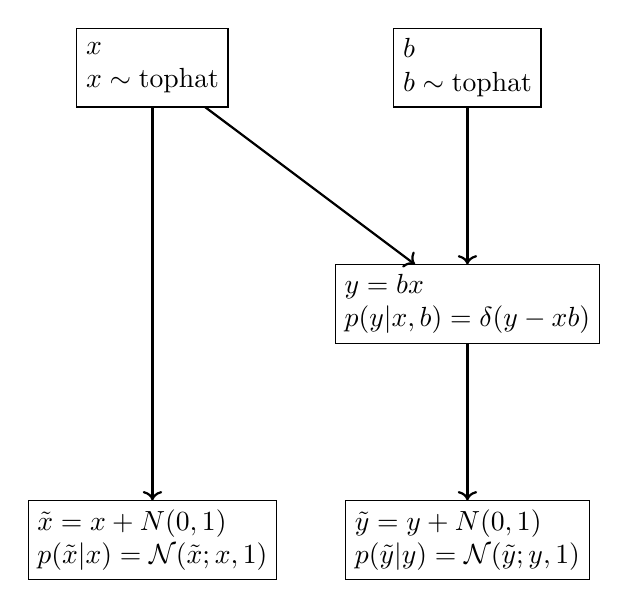
\begin{tikzpicture}[
	state/.style={draw,rectangle,minimum size=1cm,outer sep=0pt,align=left}]
	\node[state] (A) at (-2,3) {$x$ \\ $x \sim \textrm{tophat}$};
	\node[state] (B) at (2,3) {$b$ \\ $b \sim \textrm{tophat}$};
	\node[state] (C) at (2,0) {$y=bx$ \\ $p(y|x,b)=\delta(y-xb)$};
	\node[state] (D) at (-2,-3) {$\tilde{x}=x+N(0,1)$ \\ $p(\tilde{x}|x) = \mathcal{N}(\tilde{x}; x, 1)$};
	\node[state] (E) at (2,-3) {$\tilde{y}=y+N(0,1)$ \\ $p(\tilde{y}|y) = \mathcal{N}(\tilde{y}; y, 1)$};
	\draw[->, thick] (A) -- (D);
	\draw[->, thick] (B) -- (C);
	\draw[->, thick] (A) -- (C);
	\draw[->, thick] (C) -- (E);
\end{tikzpicture}
\end{frame}


\begin{frame}{Posterior}
	So now we can use Bayes's Theorem to write down the posterior. If we have written out the graph correctly, then it's just a matter of multiplying all the probabilities in the graph and integrating over any intermediate variables (and so you can skip to the third line):
	\begin{align*}
	p(b, x | \tilde{x}, \tilde{y}) &\propto  p(\tilde{x}, \tilde{y}|b, x) \ p(b) \ p(x) \\
	&\propto \int p(\tilde{x} | x) \ p(\tilde{y} | y) \ p(y | x, b) \ p(b) \ p(x) \ \mathd{}y\\
	&\propto \int \mathcal{N}(\tilde{x}; x, 1) \ \mathcal{N}(\tilde{y}; y, 1) \ \delta(y-xb) \ U(b) \ U(x) \ \mathd{}y\\ 
	&\propto \mathcal{N}(\tilde{x}; x, 1) \ \mathcal{N}(\tilde{y}; xb, 1) \ U(b) \ U(x) \\
	&\propto \exp(-\frac{1}{2} ((\tilde{x} - x)^2 + (\tilde{y} - xb)^2)) \ U(b) \ U(x) \\
	\end{align*}
\end{frame}

\begin{frame}{Get rid of the nuisance parameter}
        \begin{itemize}
    \item{This is our answer - it's the (joint) posterior distribution for $x$ and $b$ (under this model).}
    \item{But we only care about $b$! So we need to \textit{marginalise} i.e. project the probabilities from the two-dimensional $(x, b)$ parameter space down to the one-dimensional $b$ parameter space. Do this by integrating over $x$.}
    \end{itemize}
	\begin{align*}
	p(b | \textrm{data}) &\propto \int p(b, x |\textrm{data})) \ \mathd{}x \\
	&\propto \int \exp(-\frac{1}{2} ((\tilde{x} - x)^2 + (\tilde{y} - xb)^2)) \ U(b) \ U(x) \ \mathd{}x 
	\end{align*}
\end{frame}

\begin{frame}{A Useful Definite Integral}
If $A>0$ then
	\begin{equation*}
	\int_{-\infty}^{\infty} \exp(-Ax^2 +Bx+C) \ \mathd{}x = \sqrt{\frac{\pi}{A}} \exp\left(\frac{B^2}{4A} + C\right)
	\end{equation*}
	This generalises the Gaussian integral (for which $A=1$, $B=C=0$).
\end{frame}

\begin{frame}{Marginalised posterior for $b$}
Thus we get to our goal: the marginalised posterior for $b$ (under this model):
	\begin{equation*}
	p(b | \tilde{x}, \tilde{y}) \propto \frac{1}{\sqrt{1+b^2}} \exp\left( \frac{(\tilde{x}+b\tilde{y})^2}{2(1+b^2)}\right)
	\end{equation*}
        \begin{itemize}
    \item{Note a factor of $1/2$ in the exponential function, but no minus sign.}
    \item{Note the curious combination $\tilde{x}+b\tilde{y}$; you might have expected $\tilde{y}-b\tilde{x}$.}
    \end{itemize}
\end{frame}

\begin{frame}{Marginalised posterior for $b$}
	\begin{figure}
	\centering
		\includegraphics[scale=0.62]{figure_5.png}
	\end{figure}
\end{frame}

\begin{frame}{Marginalised posterior for $b$}
        \begin{itemize}
    \item{Note the (anticipated) tail to the right.}
    \item{The value $1.21$ displayed at the at the top of the plot is the \textit{mode} i.e. the value of $b$ for which the posterior probability density is maximum. Note that it's close to, but a little less than, the ratio $\tilde{b} = \tilde{y} / \tilde{x}$ seen in the data.}
    \end{itemize}
\end{frame}

\begin{frame}{Joint posterior for $b$  and $x$}
	\begin{figure}
	\centering
		\includegraphics[scale=0.62]{figure_6.png}
	\end{figure}
\end{frame}

\begin{frame}{Joint posterior for $b$  and $x$, showing $y=bx$ as well}
	\begin{figure}
	\centering
		\includegraphics[scale=0.62]{figure_7.png}
	\end{figure}
\end{frame}

\begin{frame}{Posteriors for galaxy/DM ratio from 2509.18967}
	\begin{figure}
	\centering
		\includegraphics[scale=0.38]{figure_2509_18967.png}
	\end{figure}
\end{frame}

\begin{frame}{Widening the tophat priors}
The left and right bounds on the priors for $x$ and $b$ were somewhat arbitrary. Can we get rid of these bounds, so that the prior density is the same non-zero value everywhere? Mathematically we do this by taking the limit as the bounds go to plus and minus infinity.
 \begin{itemize}
    \item{For $x$ there is no problem; the required limits exist. In fact we already assumed $-\infty < x < \infty$ when we did the marginalisation integral.}
    \item{But for $b$ we see that the posterior looks like $(1+b^2)^{-1/2}$ for large $b$; the integral of this over $0 < b < \infty$ is infinite. This is bad news for a probability distribution, as it means we can't normalise it so that the total probability (i.e. the area under the posterior function) is unity. So it's crucial to have a prior with a right-hand cutoff!}
    \end{itemize}
\end{frame}

\begin{frame}{Inference works even for a wrong model}
 \begin{itemize}
    \item{We could have used these ideas to constrain the parameters even of a wrong model.}
    \item{For example, we could have modelled the ratio as the sine of an angle $\sin(\theta) = y/x$; we would still get constraints on $\theta$.}
    \item{\textit{Bayesian model comparison} lets us separate good models from bad.}
    \end{itemize}
\end{frame}

\begin{frame}{Alternative prior}
 \begin{itemize}
    \item{The prior used so far doesn't treat $x$ and $y$ in the same way.}
    \item{The flat priors on $b$ and $x$ mean that the implied prior density of $y$ is large when $x$ is small and small when $x$ is large.}
    \item{An alternative prior would be flat on both $x$ and $y$. We can get this within our current model by setting the prior probability of $x$ to be proportional to $|x|$.}
    \item{This introduces an additional factor of $|x|$ into our posterior.}
    \item{Note that this is identical to the naive method that I tried first!}
    \end{itemize}
\end{frame}

\begin{frame}{Posterior for alternative prior}
The marginalised posterior for $b$ (under this model, using flat prior on $b$ and $|x|$ prior on $x$):
	\begin{equation*}
	p(b | \tilde{x}, \tilde{y}) \propto \frac{2}{1+b^2} + \frac{2 \sqrt{\pi} \ \Gamma}{1+b^2} \exp(\Gamma^2) \erf(\Gamma)
	\end{equation*}
	where 
	\begin{equation*}
	\Gamma = \frac{\tilde{x} + b \tilde{y}}{\sqrt{2 (1+b^2)}}
	\end{equation*}
\end{frame}


\begin{frame}{Posterior for $b$ using a prior that is flat in $x$ and $y$}
	\begin{figure}
	\centering
		\includegraphics[scale=0.62]{figure_8.png}
	\end{figure}
\end{frame}


\begin{frame}{Posterior for $b$ and $x$ (\& $y$) using prior flat in $x$ and $y$}
	\begin{figure}
	\centering
		\includegraphics[scale=0.62]{figure_9.png}
	\end{figure}
\end{frame}


\begin{frame}{Comparison: impact of prior}
	\begin{figure}
	\centering
		\includegraphics[scale=0.62]{figure_10.png}
	\end{figure}
\end{frame}



\end{document}